% Copyright 2023,2025 Kieran W Harvie. All rights reserved.

\chapter{Automatic Differentiation}
Automatic differentiation is a collection of algorithms for calculating the partial derivatives\footnote{If we have the partial derivatives then we trivially have the total derivatives as well.} of some complex given function.
A common approach is to express the given function in terms of intermediary functions with known partial derivatives.
The chain rule can then be used to combine these partial derivatives into the desired result:
\begin{center}
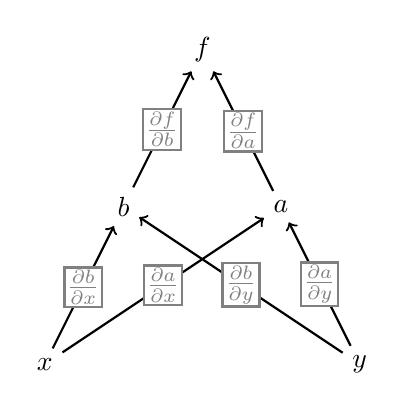
\begin{tikzpicture}
	\node (f) at (0,2) {$f$};
	\node (a) at (1,0) {$a$};
	\node (b) at (-1,0) {$b$};
	\node (x) at (-2,-2) {$x$};
	\node (y) at (2,-2) {$y$};

	\foreach \from/\to in {x/a,x/b,y/a,y/b,a/f,b/f}
		\draw[->,thick] (\from) -- (\to) node[midway,fill=white,text=gray,draw=gray,rectangle,inner sep=.1em]{$\frac{\partial \to}{\partial \from}$};
\end{tikzpicture}

	A computation graph of $f(a(x,y),b(x,y))$ where the edges are weighted according to partial derivatives. 
\end{center}
Forward and reverse accumulation are a pair of automatic differentiation algorithms where each intermediary functions has an associated accumulator.
The accumulators are used for the calculation and storage intermediary values used in the application of the chain rule.
In forward accumulation the accumulator stores the partial of its intermediary function by an input while in reverse accumulation the accumulator stores the partial of the general function by the output of its intermediary function.
Their respective names comes from the order the accumulators are used.
In forward accumulation the order matches how the intermediary functions are evaluated,
and can even be done at the same time!
In reverse accumulation the order the intermediary functions are evaluated and accumulators are used is reversed and can't be done at the same time,
although it does have other advantages to be discussed later. 
\begin{center}
\begin{tikzpicture}
	\foreach \i in {x,y,a,b,f}
		\node (\i) at (\i) {$\frac{\partial \i}{\partial x}$};
	
	\foreach \from/\to in {x/a,x/b,y/a,y/b,a/f,b/f}
		\draw[->,thick] (\from) -- (\to) node[midway,fill=white,text=gray,draw=gray,rectangle,inner sep=.1em]{$\frac{\partial \to}{\partial \from}$};
\end{tikzpicture}
\quad
\begin{tikzpicture}
	\foreach \i in {x,y,a,b,f}
		\node (\i) at (\i) {$\frac{\partial f}{\partial \i}$};
	
	\foreach \from/\to in {x/a,x/b,y/a,y/b,a/f,b/f}
		\draw[->,thick] (\to) -- (\from) node[midway,fill=white,text=gray,draw=gray,rectangle,inner sep=.1em]{$\frac{\partial \to}{\partial \from}$};
\end{tikzpicture}

	Forward (left) and reverse (right) accumulation\\
	where the nodes show what they're accumulating.
\end{center}
If you observe that each node is the sum of the nodes that point to it weighted by the edge:
\[\frac{\partial f}{\partial x} = \frac{\partial f}{\partial b}\frac{\partial b}{\partial x}+\frac{\partial f}{\partial a}\frac{\partial a}{\partial x}\]

\section{Incident Algebra Formulation}
Assume we have $\{f,F,R\}\in \Int(N,K)$ such that:
\[fF = F+R\]
Then we can expand this to get:
\[\sum_{z\in[x,y]}f[x,z]F[z,y] = F[x,y]+R[x,y]\]
If $R$ and $f[x,x]F[x,y]$ are efficient to calculate then we can use this as the basis for a method to calculate $F[x,y]$ from $\{F[z,y]\}_{z\prec x}$.
\\

This actually isn't that unlikely as if we have:
\[f[x,x] = 0 \text{ and } F = \sum_{k=0}^nf^k\]
Then
\[R=f^{n+1}-\delta\]
From double sum:
\[\begin{aligned}
	\sum_{z\in[x,y]}f[x,z]\sum_{k=0}^nf^k[z,y] =& \sum_{k=0}^n\sum_{z\in[x,y]}f[x,z]f^k[z,y]\\
	=& \sum_{k=0}^nf^{k+1}[z,y]\\
	=& \sum_{k=0}^nf^k[z,y]+f^{n+1}[x,y]-\delta[x,y]\\
\end{aligned}\]
$f$ be nilpotent:
\[f^{n+1}=0\]

\section{Example Traces}
\subsection{Forward Accumulation}
\subsection{Reverse Accumulation}
One visual trace of the is worth a thousand lines of analysis.
Let $f(x,y) = \frac{1}{2}x+y,\,a(x)=x^2,\,b(x)=x^3,$ and $x=0.5$, 
we wish to preform reverse accumulation for $f(a(x),b(x))$.

We will represent the state of the algorithm as a weighed directed graph,
the nodes are the inputs/outputs/intermediates and an accumulator,
the edge direction is downstream (from input to output),
the edge weights are the partial derivatives of the nodes.
\begin{multicols}{2}
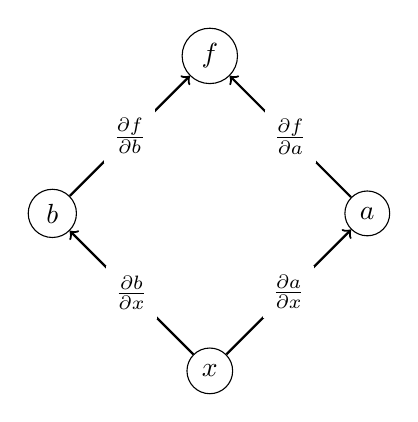
\begin{tikzpicture}
	\node[draw, circle] (f) at (0,2) {$f$};
	\node[draw, circle] (a) at (2,0) {$a$};
	\node[draw, circle] (b) at (-2,0) {$b$};
	\node[draw, circle] (x) at (0,-2) {$x$};
	
	\draw[->,thick] (x.north west) -- (b.south east) node[midway,fill=white]{$\frac{\partial b}{\partial x}$};
	\draw[->,thick] (x.north east) -- (a.south west) node[midway,fill=white]{$\frac{\partial a}{\partial x}$};
	\draw[->,thick] (a.north west) -- (f.south east) node[midway,fill=white]{$\frac{\partial f}{\partial a}$};
	\draw[->,thick] (b.north east) -- (f.south west) node[midway,fill=white]{$\frac{\partial f}{\partial b}$};
\end{tikzpicture}
	\columnbreak
	\centering
	\begin{center}
\begin{tabular}{|c|c|c|c|c|}
	\hline
	\bf Node:\phantom{\bigg|} &$x$&$a$&$b$&$f$\\
	\hline
	Value: &&&&\\
	Accumulator: &&&&\\
	\hline
	\hline
	\bf Edge:\phantom{\bigg|} &$\frac{\partial a}{\partial x}$&$\frac{\partial b}{\partial x}$&$\frac{\partial f}{\partial a}$&$\frac{\partial f}{\partial b}$\\
	\hline
	Value: &&&&\\
	\hline
\end{tabular}
	\end{center}
\end{multicols}

The first pass is forward and we calculate the values of the nodes and edges.
This is straight forward, for example, since we have $x=0.5$ and $a(x)=x^2$ the desired values are $a=0.25$ and $\frac{\partial a}{\partial x} = 1.0$
\begin{multicols}{2}
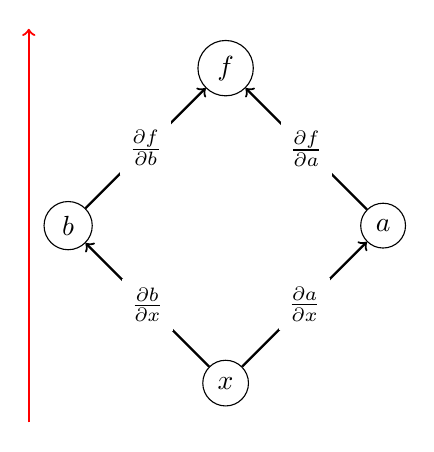
\begin{tikzpicture}
	\node[draw, circle] (f) at (0,2) {$f$};
	\node[draw, circle] (a) at (2,0) {$a$};
	\node[draw, circle] (b) at (-2,0) {$b$};
	\node[draw, circle] (x) at (0,-2) {$x$};
	
	\draw[->,thick] (x.north west) -- (b.south east) node[midway,fill=white]{$\frac{\partial b}{\partial x}$};
	\draw[->,thick] (x.north east) -- (a.south west) node[midway,fill=white]{$\frac{\partial a}{\partial x}$};
	\draw[->,thick] (a.north west) -- (f.south east) node[midway,fill=white]{$\frac{\partial f}{\partial a}$};
	\draw[->,thick] (b.north east) -- (f.south west) node[midway,fill=white]{$\frac{\partial f}{\partial b}$};
	\draw[->,red,thick] (-2.5,-2.5)--(-2.5,2.5);
\end{tikzpicture}
	\columnbreak
	\centering
	\begin{center}
\begin{tabular}{|c|c|c|c|c|}
	\hline
	\bf Node:\phantom{\bigg|} &$x$&$a$&$b$&$f$\\
	\hline
	Value: &0.5&0.25&0.125&0.25\\
	Accumulator: &&&&\\
	\hline
	\hline
	\bf Edge:\phantom{\bigg|} &$\frac{\partial a}{\partial x}$&$\frac{\partial b}{\partial x}$&$\frac{\partial f}{\partial a}$&$\frac{\partial f}{\partial b}$\\
	\hline
	Value: &1.0&0.75&0.5&1.0\\
	\hline
\end{tabular}
	\end{center}
\end{multicols}

The second pass is backwards where we set the accumulator of the output $f$ to $1$ and then recursively add the product of downstream element accumulators by edge weight to their upstream elements accumulators.

We will break this into two parts,
first part are the upstreams of the $f$ node.
The $a$ accumulator is $0.5\times1.0$ and $b$'s is $1.0\times1.0$:
\begin{multicols}{2}
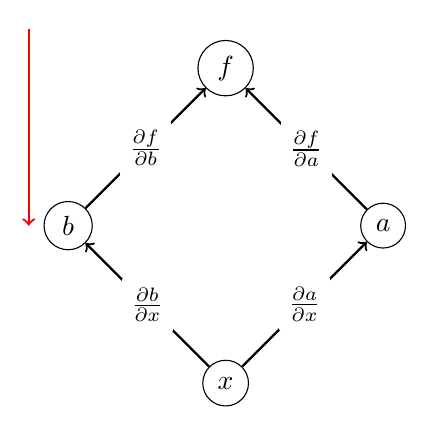
\begin{tikzpicture}
	\node[draw, circle] (f) at (0,2) {$f$};
	\node[draw, circle] (a) at (2,0) {$a$};
	\node[draw, circle] (b) at (-2,0) {$b$};
	\node[draw, circle] (x) at (0,-2) {$x$};
	
	\draw[->,thick] (x.north west) -- (b.south east) node[midway,fill=white]{$\frac{\partial b}{\partial x}$};
	\draw[->,thick] (x.north east) -- (a.south west) node[midway,fill=white]{$\frac{\partial a}{\partial x}$};
	\draw[->,thick] (a.north west) -- (f.south east) node[midway,fill=white]{$\frac{\partial f}{\partial a}$};
	\draw[->,thick] (b.north east) -- (f.south west) node[midway,fill=white]{$\frac{\partial f}{\partial b}$};
	\draw[->,red,thick] (-2.5,2.5)--(-2.5,0);
\end{tikzpicture}
	\columnbreak
	\centering
	\begin{center}
\begin{tabular}{|c|c|c|c|c|}
	\hline
	\bf Node:\phantom{\bigg|} &$x$&$a$&$b$&$f$\\
	\hline
	Value: &0.5&0.25&0.125&0.25\\
	Accumulator: &&0.5&1.0&1.0\\
	\hline
	\hline
	\bf Edge:\phantom{\bigg|} &$\frac{\partial a}{\partial x}$&$\frac{\partial b}{\partial x}$&$\frac{\partial f}{\partial a}$&$\frac{\partial f}{\partial b}$\\
	\hline
	Value: &1.0&0.75&0.5&1.0\\
	\hline
\end{tabular}
	\end{center}
\end{multicols}

And then we add continue to add the product of accumulator by edge weight to upstream nodes.
The only upstream node left is $x$ and in hence set to $0.5\times1.0+1.0\times0.75$:
\begin{multicols}{2}
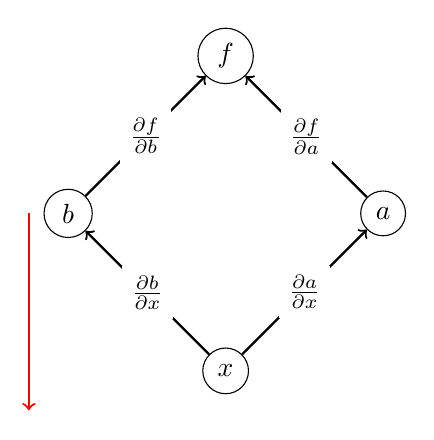
\begin{tikzpicture}
	\node[draw, circle] (f) at (0,2) {$f$};
	\node[draw, circle] (a) at (2,0) {$a$};
	\node[draw, circle] (b) at (-2,0) {$b$};
	\node[draw, circle] (x) at (0,-2) {$x$};
	
	\draw[->,thick] (x.north west) -- (b.south east) node[midway,fill=white]{$\frac{\partial b}{\partial x}$};
	\draw[->,thick] (x.north east) -- (a.south west) node[midway,fill=white]{$\frac{\partial a}{\partial x}$};
	\draw[->,thick] (a.north west) -- (f.south east) node[midway,fill=white]{$\frac{\partial f}{\partial a}$};
	\draw[->,thick] (b.north east) -- (f.south west) node[midway,fill=white]{$\frac{\partial f}{\partial b}$};
	\draw[->,red,thick] (-2.5,0)--(-2.5,-2.5);
\end{tikzpicture}
	\columnbreak
	\centering
	\begin{center}
\begin{tabular}{|c|c|c|c|c|}
	\hline
	\bf Node:\phantom{\bigg|} &$x$&$a$&$b$&$f$\\
	\hline
	Value: &0.5&0.25&0.125&0.25\\
	Accumulator: &1.25&0.5&1.0&1.0\\
	\hline
	\hline
	\bf Edge:\phantom{\bigg|} &$\frac{\partial a}{\partial x}$&$\frac{\partial b}{\partial x}$&$\frac{\partial f}{\partial a}$&$\frac{\partial f}{\partial b}$\\
	\hline
	Value: &1.0&0.75&0.5&1.0\\
	\hline
\end{tabular}
	\end{center}
\end{multicols}

The algorithm has completed and in the accumulator of each node is the partial derivative of $f$ by that node.
For example $\frac{\partial f}{\partial x} = 1.25,\,\frac{\partial f}{\partial a} = 0.5,\,\frac{\partial f}{\partial b} = 1.0,$ and $\frac{\partial f}{\partial f} = 1.0$.
